\section{Exercises}
\renewcommand{\arraystretch}{1.5}
\subsection*{Neural Network}
\subsubsection*{Exercise 1}
Consider the following neural network which takes two binary-valued inputs $x_1,x_2 \in {0,1}$ and outputs $h_\theta(x)$. Which of the following logical function does it compute?
\begin{figure}[htbp]
    \centering
    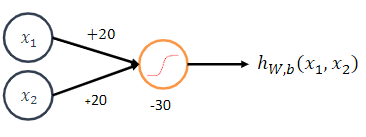
\includegraphics[width=10cm]{ExerciseBook/01-NeuralNetwork/exercise1.png}\newline
\end{figure}\newline
To anser we can simply compute the truth table for the possible values of $x_1, x_2$.
\begin{center}
    
    \begin{tabular}{ |c |c |c |}
        \hline
        \textbf{$x_1$} & \textbf{$x_2$} & \textbf{$h_{W,b}(x_1,x_2)$} \\
        \hline
        0 & 0 & -30 (0) \\ 
        0 & 1 & -10 (0) \\  
        1 & 0 & -10 (0) \\
        1 & 1 & 10 (1)\\
        \hline
    \end{tabular}
    Answer: logical AND
\end{center}
\subsubsection*{Exercise 2}
Consider the following neural network:
\begin{figure}[htbp]
    \centering
    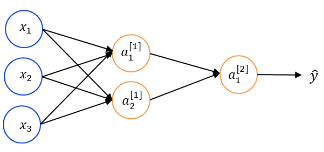
\includegraphics[width=10cm]{ExerciseBook/01-NeuralNetwork/exercise2.png}\newline
\end{figure}
I start by computing the activation vector $z^{[1]}$ by multiplying $W\cdot x+b^{[1]}$.
\[ 
    z^{[1]}=
    \begin{bmatrix}
        -1 \\
        8 
    \end{bmatrix}
\]
\\I then plug the activation vector into the activation function to get $a^{[1]} = g(z^{[1]}) = \frac{1}{1-e^{-z^{[1]}}}$
\[ 
    a^{[1]}=
    \begin{bmatrix}
        0.268941 \\
        0.999665
    \end{bmatrix}
\]\\I repeat for the next layer
\[ 
    z^{[2]}=
    \begin{bmatrix}
        2.537547
    \end{bmatrix}
\]
\\We conclude $a^{[2]}=0.926732$
\subsubsection*{Exercise 3}
\begin{figure}[htbp]
    \centering
    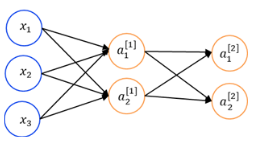
\includegraphics[width=10cm]{ExerciseBook/01-NeuralNetwork/exercise3.png}\newline
\end{figure}
I start by computing the activation vector $z^{[1]}$ by multiplying $W\cdot x+b^{[1]}$.
\[ 
    z^{[1]}=
    \begin{bmatrix}
        4 \\
        -16
    \end{bmatrix}
\]
\[ 
    a^{[1]}=
    \begin{bmatrix}
        0.982014 \\
        0.00000012 \\ 
    \end{bmatrix}
\]
\[ 
    z^{[2]}=
    \begin{bmatrix}
        2.964028 \\
        3.964027
    \end{bmatrix}
\]
\[ 
    a^{[2]}=
    \begin{bmatrix}
        0.268941 \\
        0.731058
    \end{bmatrix}
\]
\subsubsection*{Esercise 4}
In this diagram which we hand-drew in lecture, what do the horizontal axis (x-axis) and vertical axis (y-axis) represent?
\begin{figure}[htbp]
    \centering
    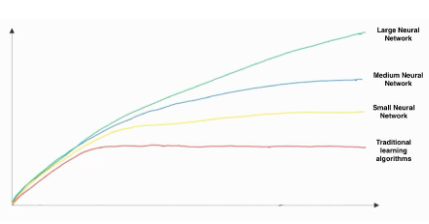
\includegraphics[width=10cm]{ExerciseBook/01-NeuralNetwork/exercise4.png}\newline
\end{figure}
Answer: x-axis is the amount of data; y-axis (vertical axis) is the performance of the algorithm.
\subsubsection*{Exercise 5}
Which one of these plots represents a ReLU activation function?
\begin{figure}[htbp]
    \centering
    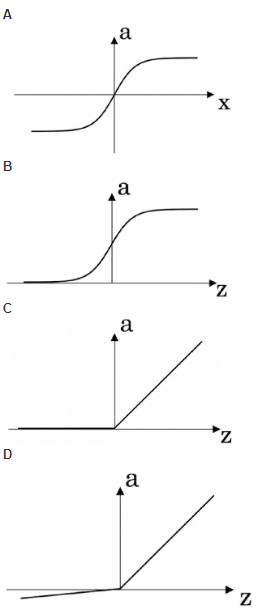
\includegraphics[width=6cm]{ExerciseBook/01-NeuralNetwork/exercise5.png}\newline
\end{figure}
Solution answer C
\subsubsection*{Exercise 6}
Which of these is the "Logistic Loss"?\\
Solution answer A
\subsubsection*{Exercise 7}
Consider the following computation graph. What is the output J?
\begin{figure}[htbp]
    \centering
    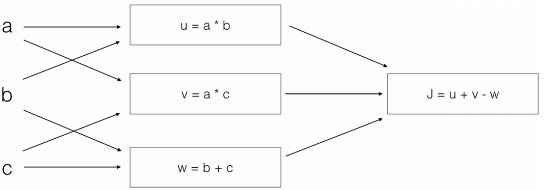
\includegraphics[width=6cm]{ExerciseBook/01-NeuralNetwork/exercise7.png}\newline
\end{figure}
Solution answer B
\subsubsection*{Exercise 8}
You are building a binary visual classifier for recognizing apples(y=1) vs. tomatoes(y=0). Which one of these activation functions would yourecommend using for the output layer?
\\Solution: answer C and D: Sigmoid and Tanh, because they are perfect for linear classification
\subsubsection*{Exercise 9}
Suppose you have built a neural network. You decide to initialize the weights and biases to be zero. Which of the following statements is true?\\
Solution answer A: Each neuron in the first hidden layer will perform the same computation. So even after multiple iterations of gradient descent each neuron in the layer will becomputing the samething as other neurons.
\subsubsection*{Exercise 10}
Consider the following 2 hidden layer neural network, which of the following statements are True?
\begin{figure}[htbp]
    \centering
    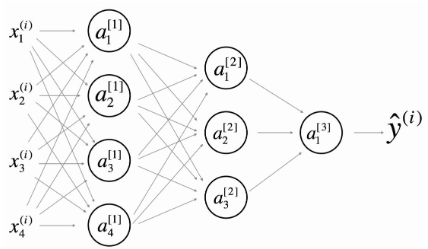
\includegraphics[width=6cm]{ExerciseBook/01-NeuralNetwork/exercise10.png}\newline
\end{figure}
Solution, answers A, B, F
\subsubsection*{Exercise 11}
The dev and test set should:
Solution answer A: come from the same distribution.
\subsubsection*{Exercise 12}
If your Neural Network model seems to underfit your data, what of the following would be promising things to try?\\
Solution answers: B, C, D